\documentclass[tikz,border=2mm]{standalone}
\usepackage{tikz}
\usetikzlibrary{arrows}
\usetikzlibrary{arrows.meta,automata,positioning}

\begin{document}

% \usetikzlibrary{arrows.meta,automata,positioning}
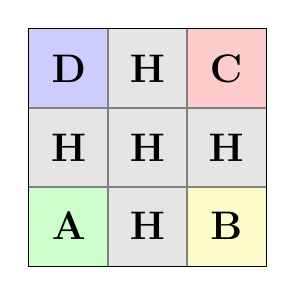
\begin{tikzpicture}

% Draw the outer walls (thick lines)
\draw[very thick] (0,0) rectangle (3,3);
\fill[blue!20] (0,2) rectangle (1,3); % Room D
\fill[green!20] (0,0) rectangle (1,1); % Room A
\fill[red!20] (2,2) rectangle (3,3); % Room C
\fill[yellow!20] (2,0) rectangle (3,1);
\fill[gray!20] (1,0) rectangle (2,1);
\fill[gray!20] (1,1) rectangle (2,2);
\fill[gray!20] (1,2) rectangle (2,3);
\fill[gray!20] (0,1) rectangle (1,2);
\fill[gray!20] (2,1) rectangle (3,2);

Draw the inner walls (gray lines)
\draw[gray, thick] (2,0) -- (2,3);
\draw[gray, thick] (0,2) -- (3,2);
\draw[gray, thick] (1,0) -- (1,3);
% \draw[gray, thick] (3,0) -- (3,3);
\draw[gray, thick] (0,1) -- (3,1);
% \draw[gray, thick] (0,3) -- (3,3);

% % Labels for rooms
\node at (0.5, 2.5) {\Large\textbf{D}};
\node at (0.5, 0.5) {\Large\textbf{A}};
\node at (2.5, 2.5) {\Large \textbf{C}};
\node at (2.5, 0.5) {\Large \textbf{B}};
\node at (1.5, 0.5) {\Large \textbf{H}};
\node at (1.5, 1.5) {\Large \textbf{H}};
\node at (1.5, 2.5) {\Large \textbf{H}};
\node at (0.5, 1.5) {\Large \textbf{H}};
\node at (2.5, 1.5) {\Large \textbf{H}};

\end{tikzpicture}


\end{document}